%source: Path: /mnt/9636D17436D15639/University/Ta/Logic/Design/Utils/Adel/hw4_solutions.pdf

مدار نشان داده شده در شکل زیر، T فلیپ‌فلاپ \lr{Master-Slave} است. با فرض اینکه فلیپ‌فلاپ‌ها در حالت اولیه، \lr{Reset} هستند، خروجی‌های \lr{Q} و \lr{Q'} را بدون درنظر گرفتن تاخیر‌ها، به‌ازای سیگنال کلاک و T زیر رسم کنید. \newpage


\begin{figure}[h]
	\centering
	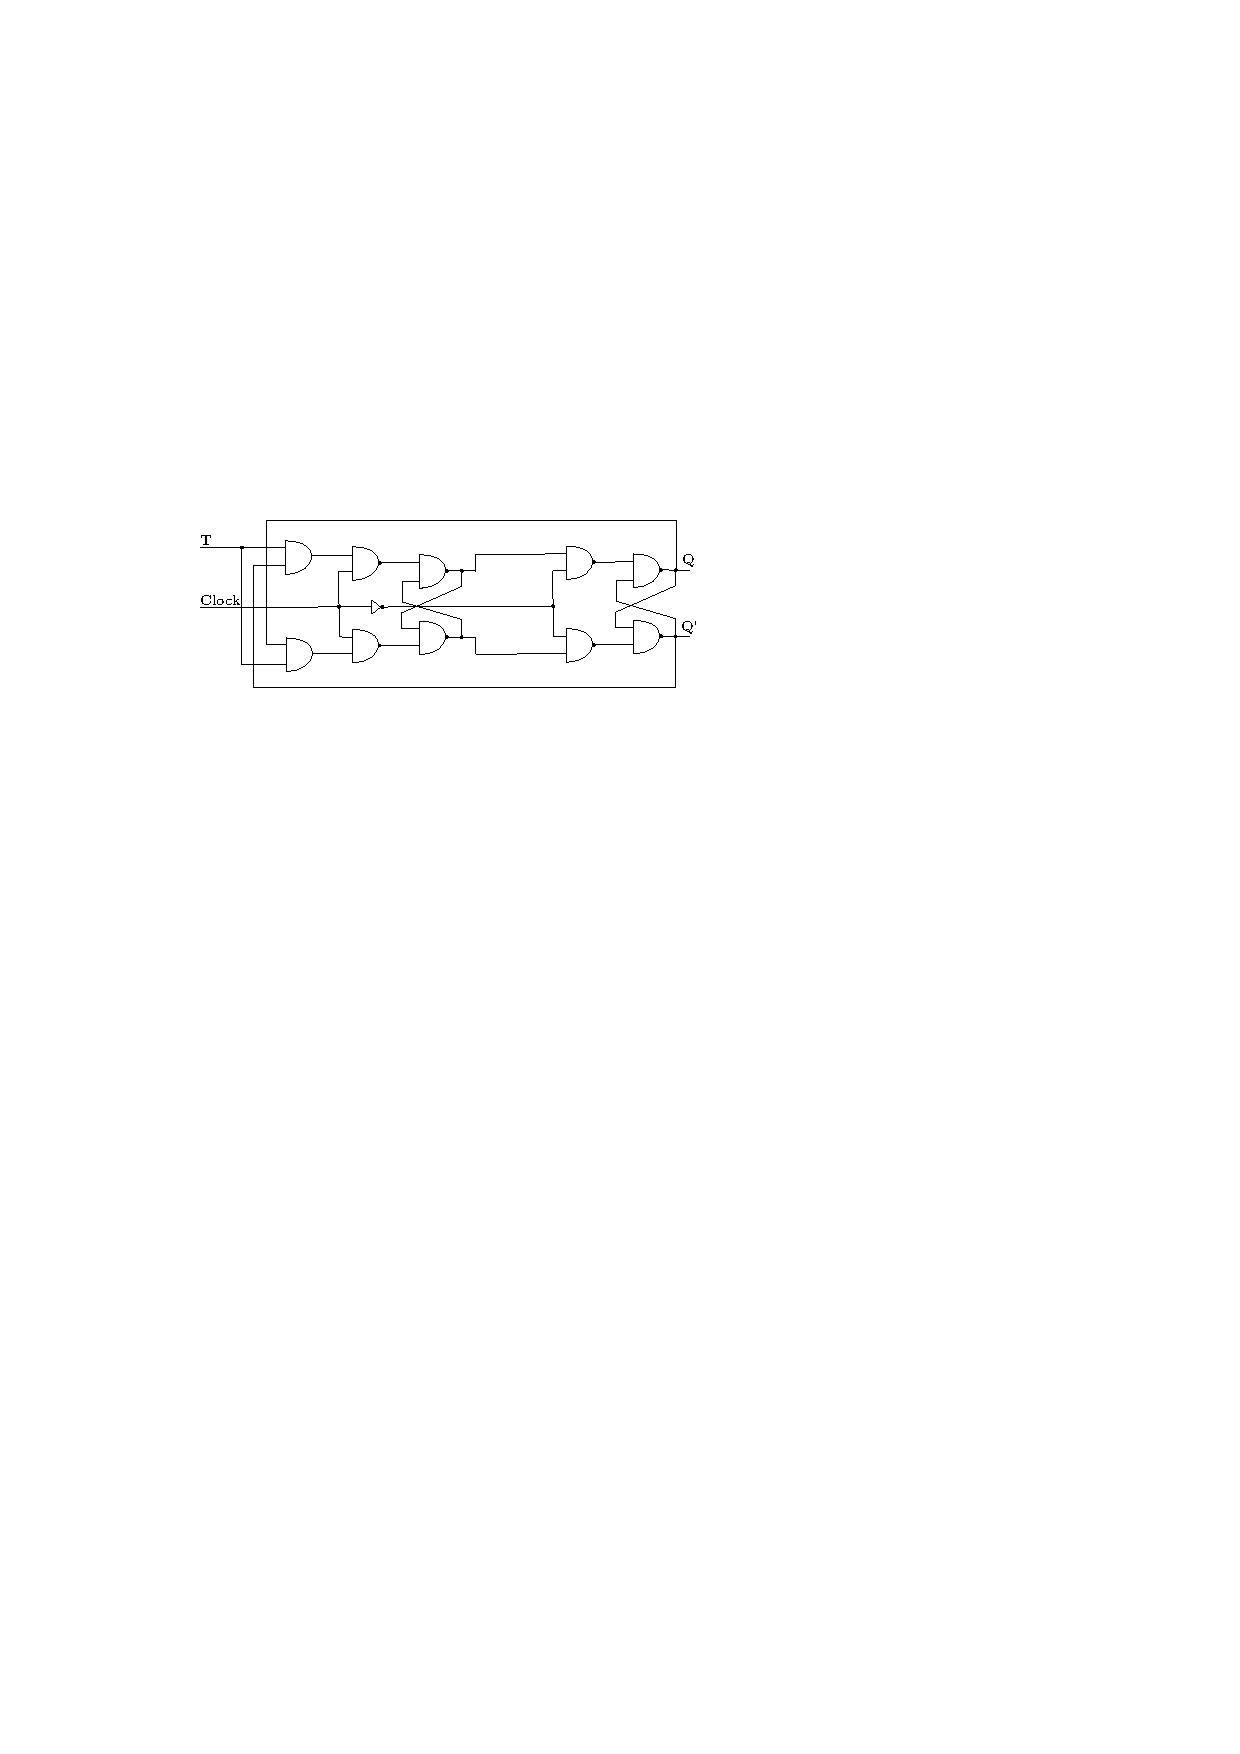
\includegraphics[width=0.8\textwidth]{fig/Q_opt2.pdf}
	\label{fig:Q_opt_2}
\end{figure}

\begin{figure}[h]
	\centering
	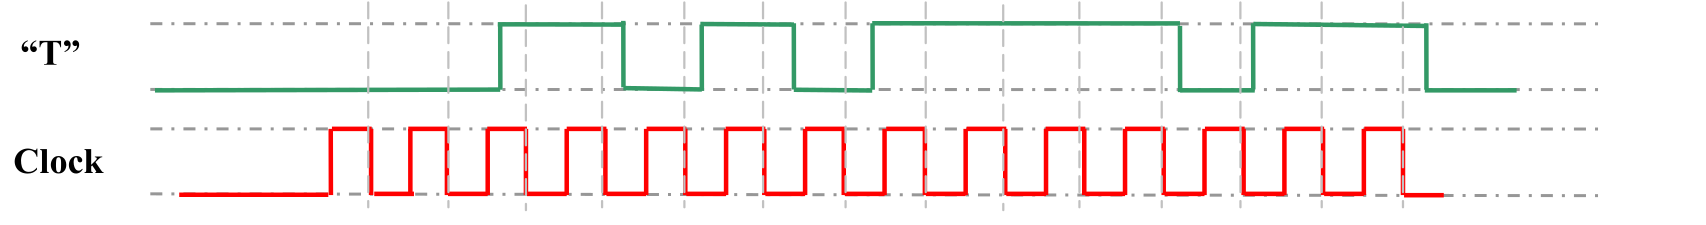
\includegraphics[width=1\textwidth]{fig/Q_opt2_2.png}
	\label{fig:Q_opt_2_2}
\end{figure}







%source: AUT-CE-LC HW10-Q2

%خروجی \lr{Q} لچ \lr{D} را با توجه به سیگنال ورودی داده شده رسم کنید.
%
%\begin{figure}[h]
%	\centering
%	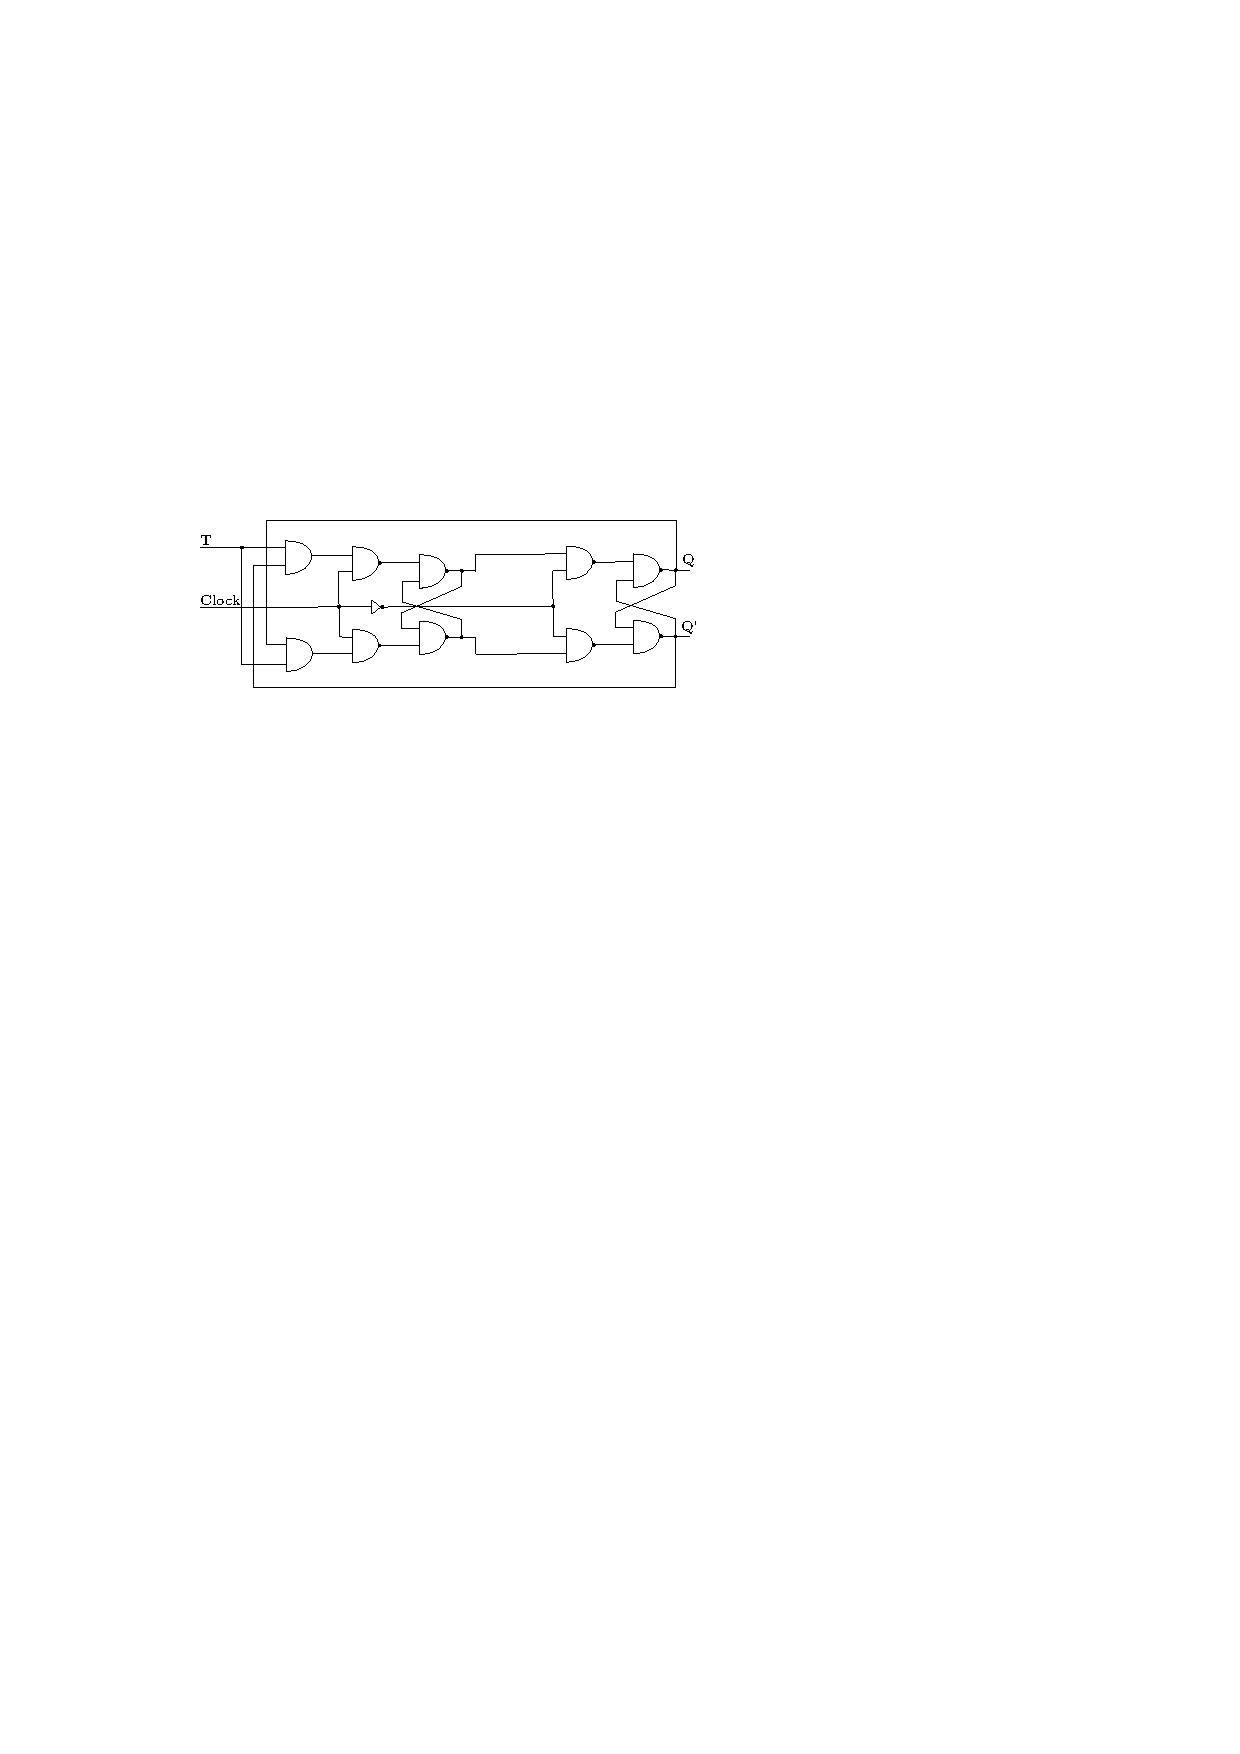
\includegraphics[width=0.6\textwidth]{fig/Q_opt2.pdf}
%	\label{fig:Q_opt_2}
%\end{figure}